\section{How a Medium Absorbs Intelligence}

The same output rate can mean abundance in one setting and overload in another. The difference lies in what must happen after the output arrives.

\subsection{Three Response Patterns}

\subhead{Bits: diffusion and replication}

Digital output can be copied and transmitted with little additional handling per recipient. A patch, image, or document can therefore spread rapidly. Once it enters a shared state, a production process, or a decision, its failure costs change.

Digital traffic can also outrun a channel. Congestion-control work treats the network's capacity and feedback as part of the sending problem.\cite{jacobson1988} A sender that can create more packets has not established that more packets will arrive usefully.

Generated material introduces an evidential version of the same issue. More records can make source tracking and quality control harder. Research on recursive training with generated data identifies conditions under which a distribution can deteriorate; it does not establish that every use of synthetic data must fail.\cite{shumailov2024ai}

\subhead{Atoms: work and sequential operations}

A manufactured output has to pass through actual operations. Some are parallelizable, others form a critical path. Adding plans does not automatically add machines, crews, feedstock, or a heat-removal path.

A production line can respond with an initial delay followed by a limited rate of output. Once a demand fits its capacity, a more intelligent schedule can help. Above capacity, priorities, queues, rejection, and investment determine what happens next.

\subhead{Life: response to an intervention}

A living system responds through regulation, compensation, adaptation, and multiple timescales. A dose changes concentrations, which change interactions, which can alter the subsequent response. The action enters a system already maintaining itself.

Shear thickening in suspensions provides a physical image of resistance that can rise with the rate of imposed deformation.\cite{brown2014shear} Biological and social resistance need their own mechanisms and measurements. The image directs attention toward a rate-dependent response.

Three elementary curves illustrate possible response shapes:

\begin{align}
y_b(t)&=y_\infty(1-e^{-t/\tau_b}),\label{eq:resp-bit}\\
y_a(t)&=y_\infty\min\left\{\frac{(t-t_d)_+}{\tau_a},1\right\},\label{eq:resp-atom}\\
y_l(t)&=y_\infty\left[1-e^{-\zeta\omega_n t}
\left(\cos\omega_dt+\frac{\zeta}{\sqrt{1-\zeta^2}}\sin\omega_dt\right)\right],
\label{eq:resp-life}
\end{align}

where $\omega_d=\omega_n\sqrt{1-\zeta^2}$ and $0<\zeta<1$ for the third curve. The first is a first-order approach, the second a delayed rate-limited completion, and the third an underdamped second-order response.

They are worked examples, with parameters to be fitted for a chosen process. A digital migration can be slow, a physical relay very fast, and a biological response overdamped. The medium suggests questions about the mechanism; it does not assign the curve.

\subsection{Mismatch at the Interface}

\subhead{A useful signal needs a receiving capacity}

Electrical engineering gives a precise case of mismatch. For a lossless line of real positive characteristic impedance $Z_0$ terminated by a load $Z_L$,

\begin{equation}
\Gamma=\frac{Z_L-Z_0}{Z_L+Z_0},
\qquad
\frac{P_{\mathrm{refl}}}{P_{\mathrm{in}}}=|\Gamma|^2.
\end{equation}

Matching removes reflection under the stated conditions. An AI interface has different variables, so its wasted outputs cannot simply be assigned this electrical coefficient. Their measurable forms include discarded work, waiting, repeated replanning, and damage.

Let $r=v_{\mathrm{in}}/v_{\mathrm{abs}}$ compare an arrival rate with absorption capacity in the same units. An illustrative effective-progress response is

\begin{equation}
u(r)=
\begin{cases}
r,&0\leq r\leq1,\\
1-\kappa(r-1)^m,&r>1,
\end{cases}
\qquad \kappa>0,\quad m>0.
\label{eq:rate-mismatch}
\end{equation}

Below capacity, added input can increase progress. Above it, an overload penalty can offset the gain and, if damage is included in net progress, make it negative. The curve proposes a response to test. A pure queue with no damage instead produces waiting and a saturated service rate.

\subhead{Fit the interface to the task}

The practical choices are selective admission, buffering, a stable command interval, parallel receiving capacity, and a route for feedback. Their value depends on the process.

A contact controller needs fast local sensing and correction. A high-level language model can choose a task while a local policy maintains a grip. A laboratory system can generate candidates freely while admitting only a funded and informative selection to experiments.

The interface decides how intelligence becomes load. Designing it is part of building an intelligent system.

\begin{figure}[ht]
\centering
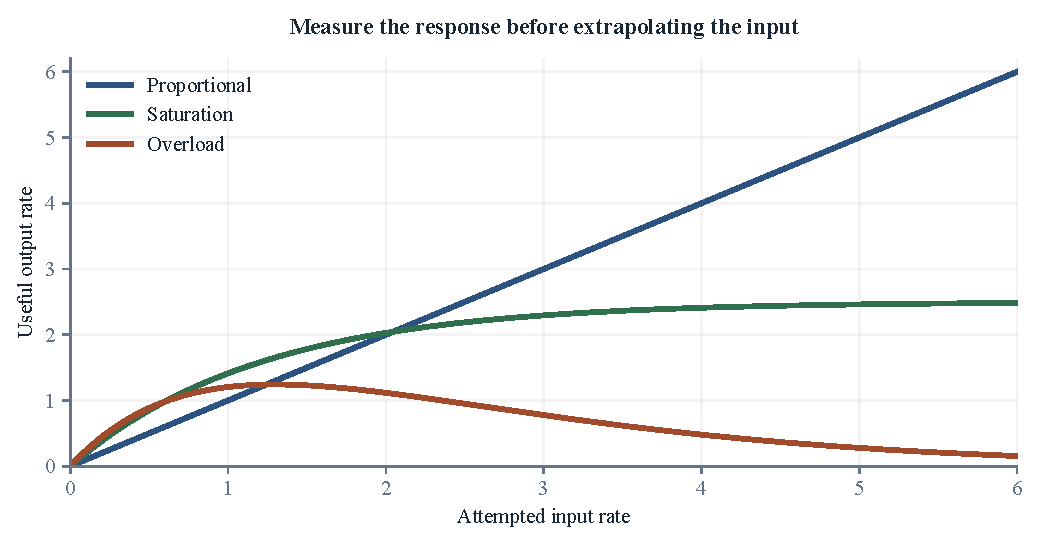
\includegraphics[width=\textwidth]{assets/response-regimes.pdf}
\caption{Useful output can scale with input, saturate, or fall under overload. These are illustrative response forms; measurements determine the form and parameters of a particular system.}
\label{fig:mechanism-response-regimes}
\end{figure}
